\chapter{Design Details}\label{Lit:desDetails}

\section{LM317 Regulation}
\label{sec:regulation}
The voltage regulation as well as the current limiting feature can be achieved with the LM317 regulator with the use of an application circuit. The LM317 is a linear regulator which means that it uses linear components such as resistors to achieve required variations, thus it is constantly dissipating power. A switching regulator makes use of PWM  to get the required variation. Because PWM means it is turns on and off it dissipates less power than a linear regulation \cite{SvsL}. Figure \ref{fig:app} is the application circuit that will be used in the design process to achieve the constant voltage and current limiting specifications. The resistor values will be redesigned. The regulator works on the basis that the difference between the output terminals and adjust terminals is a "fixed" voltage. The current flowing into $I_{adj}$ is typically 50\textmu{}A but can be a maximum of 100 \textmu{}A\cite{STM}.
The following equation \ref{eq:vo} is obtained from the data sheet \cite{STM} and correspond to figure  \ref{fig:app}.

\begin{equation}
    V_{O-reg}=V_{ref-reg}\times(1+\frac{R_2}{R_1})+(I_{adj})\times (R_2)
    \label{eq:vo}
\end{equation}

    \begin{equation}
         V_{O-reg}-V_{adj}=1.25V
         \label{eq:vref}
    \end{equation}

\subsection{Voltage regulation}
A voltage of 7.2V is designed for using equation \ref{eq:vo}. This voltage is slight lower than the 7.35V  ($2.45\times3$) specified in the data sheet. It can be considered a safety factor.  
\begin{center}
    $\frac{R_2}{R_1}=\frac{7.2}{1.25}-1=4.76$
\end{center}

The resistor values used should be kept low so that the current flowing through $R_1$ and $R_{2}$ is significantly larger than $I_{adj}$. If this is done then $I_{adj}$ can be neglected. $R_{2}$ is chosen to be 1000\textohm. Therefore $R_{1}$ will be 210\textohm. Refer to figure \ref{fig:app}.


\begin{center}
    
    $\frac{7.2}{R_1+R_2} = 6mA>>$100\textmu A
\end{center}
Because 5mA is 50 times larger than the maximum, the $I_{adj}$ can be assumed to be negligible as it will have minimal effect on the calculations.

\subsection{Current limit}

The current limiting was implemented by calculating a value for $R_4$ (refer to \ref{fig:circuit}). The maximum current that was designed for was 400mA. This value was chosen because the battery data sheet recommends 0.1C for charging which equates to 400mA \cite{RS}. This current will be designed flow when the battery is at its depleted voltage of 6V. To determine $R_s$ $V_O$ must be calculated when $V_{bat}$=6V. Using the calculated $V_0$ the resistor $R_s$ is designed for the desired current.



\begin{center}
 $V_{schottky}=0.4V$

\end{center}
\begin{center}

    $V_{adj} = (6+V_{schottky})-\frac{(6+V_{schottky})\times R_1}{R_1+R_2}$=5.29V
 
\end{center}
\begin{center}

    $V_{O-reg}= 1.25+V_{adj}$=6.539V (refer to equation \ref{eq:vref})
    
    
\end{center}
\begin{center}
    $R_s=\frac{V_{O-reg}-(V_{bat}+V_{schottky})}{400mA}=\frac{6.539V-6.4V}{300mA}=0.347$\textohm
\end{center}
The biggest flaw with this method is that $V_{schottky}$ voltage is not accurate. Another problem will be that achieving a resistance of 0.347\textohm \ will be very inaccurate.

%%%%%%%%%%%%%%%%%%%%%%%%%%%%%%%%%%%%%%%%%%%%%%
\subsection{Thermal analysis}
\begin{wrapfigure}{l}{0.25\textwidth}
\centering
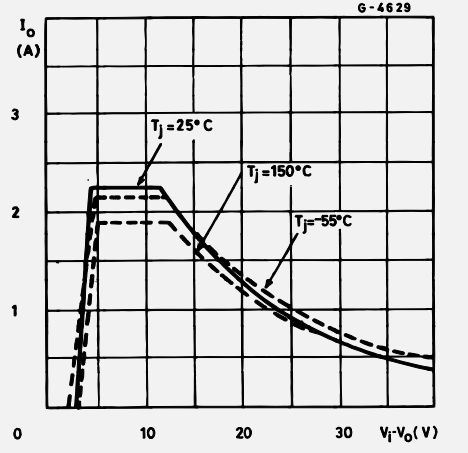
\includegraphics[scale=0.2]{Figures/temp.png}
\caption[{Output current vs. input-output
differential voltage for different junction temperatures}]{Output current vs. input-output
differential voltage for different junction temperatures\cite{STM}}
\label{fig:temp}
\end{wrapfigure}

As the junction temperature increases the output current will decrease for the same $V_i-V_{O-reg}$\cite{STM} (refer to \ref{fig:temp}). All thermal resistance values used can be found at \ref{tab:Thermal values}.



\begin{equation}
    T_j-T_a=P_{tot}\times(\theta_{j-a})
    \label{eq:woSink}
\end{equation}

\begin{equation}
    T_j-T_a=P_{tot}\times(\theta_{j-s}+\theta_{s-a})
    \label{eq:wSink}
\end{equation}

The most power our regulator will dissipate is:
\begin{center}
    $0.3A\times(12V-6.539V)=1.64W$
\end{center}


Without a heat sink, at an ambient temperature of 25\textdegree C the junction temperature will be(refer to eq. \ref{eq:woSink}):

\begin{center}
$T_j=1.64W\times(50$\textdegree C/W$)+25$\textdegree C=107\textdegree C. 
\end{center}

With the heat sink, at an ambient temperature of 25\textdegree C the junction(refer to eq. \ref{eq:wSink}):
\begin{center}
    $T_j=1.64W\times((5+20)$\textdegree C/W$)+25$\textdegree C=66\textdegree.
\end{center}

We want out current to be predictable and close to the value calculated, the heat sink enables the calculation to be more accurate. The maximum operating temperature of the regulator is 125\textdegree C \cite{STM}. 107\textdegree C is quite close and I would definitely recommend that the heat sink is used. For a higher input voltage the regulator could break without a heat sink. 


\begin{figure}[!htb]
\centering
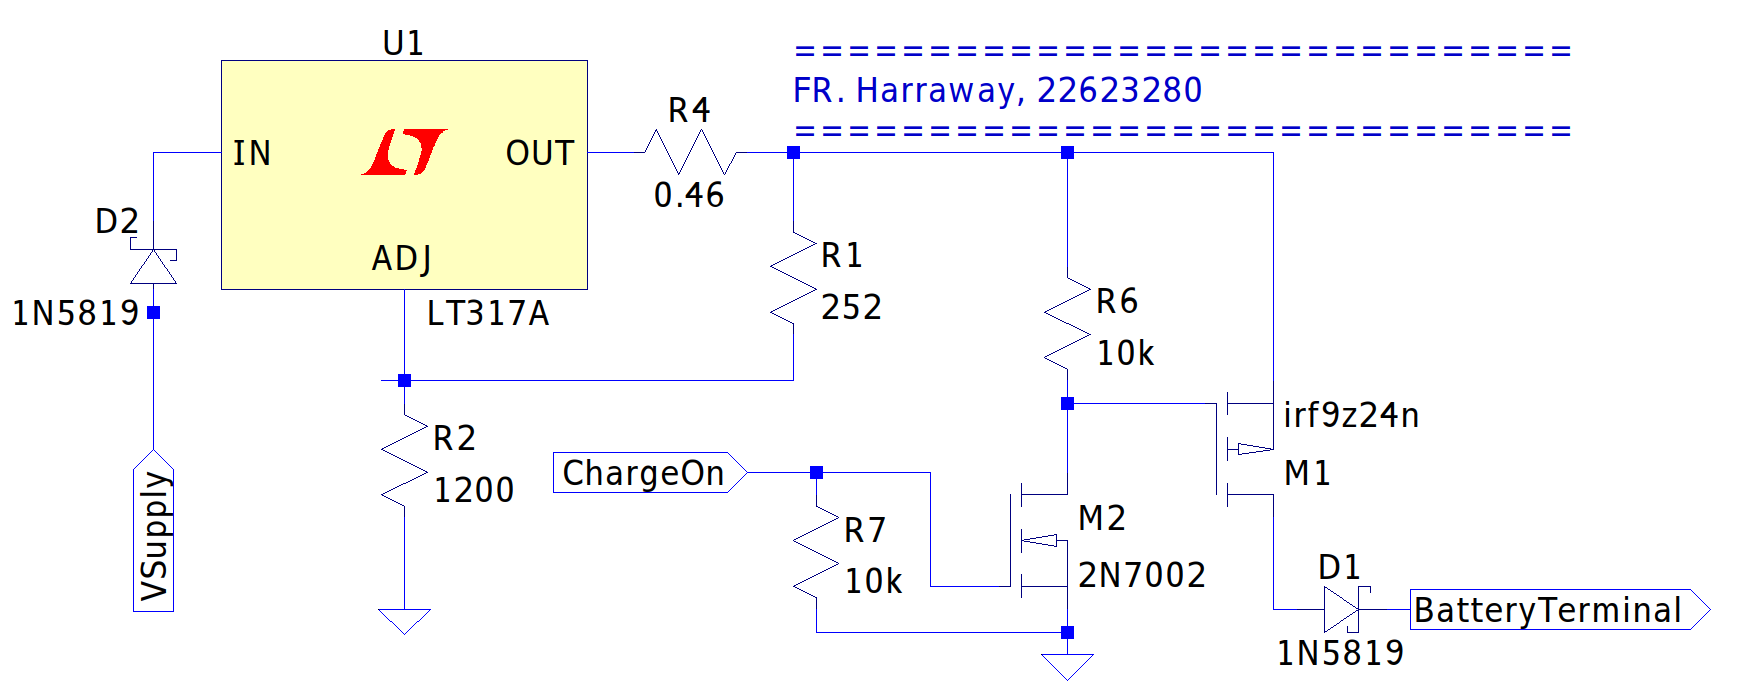
\includegraphics[scale=0.3]{Figures/FinCirc.png}
\caption{Charging Circuit with high side switch implemented }
\label{fig:circuit}
\end{figure}

%%%%%%%%%%%%%%%%%%%%%%%%%%%%%%%%%%%%%%%%%%%%%%%%%%%%%%%%%%%%%%%%%%%%%%%%%%%%%%%%%%%%%%%%%%%%%%%%%%%%%%%%%%%%%%%%%%%%%%%%%%%%%%%%%%%%%%%%%%%%%%%%%%%%%%%%%%%%%%%%%%%%%%%%%%%%%%%%%%%%%%%%%%%%%%%%%%%%%%%%%%

\section{High side switch on supply side}
\label{sec:high}
%%%second part
Switches are often used to control the flow of current within a circuit. In this report only enhancement mode MOSFETs will be used. The MOSFETs we are using have 3 terminals, gate, source and drain as can be seen in figure \ref{fig:mosfets}.\begin{wrapfigure}{l}{0.5\linewidth}
\centering
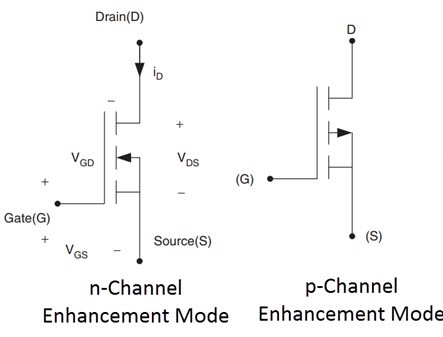
\includegraphics[height=4cm]{Figures/mosfetX.jpg}
\caption{The different MOSFET configurations}
\label{fig:mosfets}
\end{wrapfigure} For a NMOS chip the current will flow from the drain to source when it is in its \textbf{ON} state whereas for a PMOS the drain current will flow from the source to the drain. For the NMOS to turn on a positive voltage across the gate and the source must be applied that is larger than a certain threshold (refer to figure \ref{subfig:NMOS-graph}). For a PMOS the same is true however the voltage is instead negative (refer to figure \ref{subfig:PMOS-graph}).



\begin{figure}[!htb]
 \footnotesize
 \centering
    \begin{subfigure}[]{0.55\textwidth}
              \centering
  		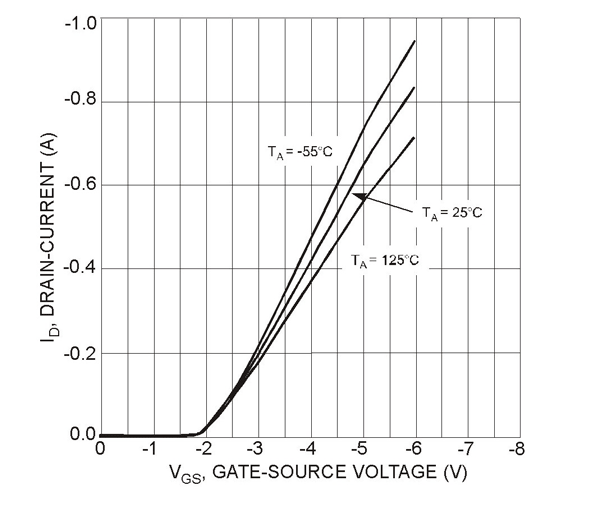
\includegraphics[width=0.5\linewidth]{./Figures/PMOS.png}
		    \caption{} \label{subfig:PMOS-graph}
     \end{subfigure}
     \begin{subfigure}[]{0.4\textwidth}
             \centering
  		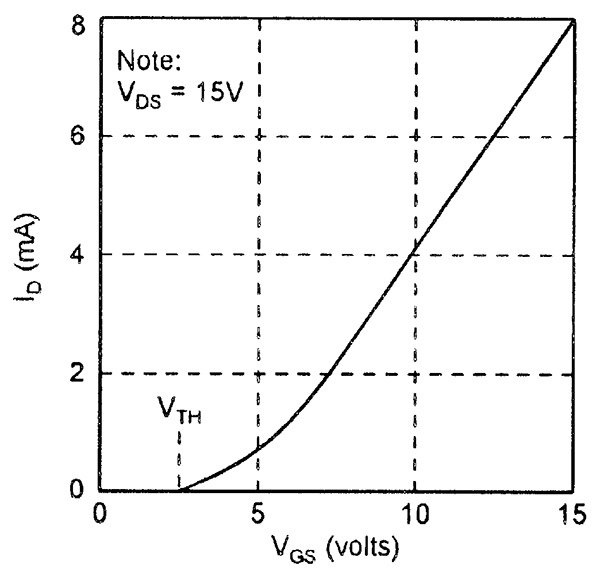
\includegraphics[width=0.6\linewidth]{./Figures/NMOS.jpg}
		   \caption{ } \label{subfig:NMOS-graph}
     \end{subfigure}
   \caption[{$V_{GS}$  vs  $I_{D}$}]{Turn on voltages for NMOS and PMOS (a)  PMOS \cite{PMOS}(b)  NMOS\cite{NMOS}  }
    \label{fig:simulation_results_box}
 \end{figure}




 When designing the switch the considerations taken into account was the fact that the PMOS can handle in excess of amps \cite{PMOS} whereas the NMOS can only handle 200mA\cite{NData}. For this reason the NMOS is used to switch the PMOS on. The way that this is achieved is by turning the NMOS on with a logic high of 5V, when the NMOS is on current flows through $R_1$ and $R_2$ (refer to figure \ref{fig:high}) and this causes there to be a voltage over the source and gate of the PMOS. This voltage needs to be greater than 4V and less than 20V in order for the PMOS to turn on and function without breaking \cite{PMOS}.The NMOS has a maximum threshold voltage of 3V. The 5V will be enough to turn it on \cite{NMOS}. A resistor is also placed between the gate of the NMOS and ground to prevent the gate from floating. 
 
\begin{itemize}
 \item To prevent current from the load from flowing back into the supply a schottky diode is placed in series with the load.
\item To ensure that all the 25V is not across the PMOS $V_{SGp}$ terminals the voltage is divided using $R_1$ and $R_2$ (refer to figure \ref{fig:high}).
\item The magnitudes of the resistors used were decided mainly to restrict excessive current flow through the resistors,$\frac{5}{10k}$=0.5mA or $\frac{25}{20k}$=1.25mA which is relatively small.
\end{itemize}



    \begin{equation}
        I_{Dn}=\frac{R_1+R_2}{V_{supply}-V_{DSn}}
        \label{eq:curr}
    \end{equation}

\begin{equation}
V_{SGp}=V_{R1}=I_{Dn}*R_1   
\label{eq:one}
\end{equation}



    $R_{1}=10k$\si{\ohm} \ $R_{2}=10k$\si{\ohm}\ $V_{supply}=25V$. If $V_{DSn}\approx0 $ for $ V_{GSn}=5V$  then using eq.\ref{eq:curr} $I_{Dn}=1.25mA$.Using eq.\ref{eq:one} $V_{SGp}=12.5V$\ , this is larger than 4V and smaller than 20V and will "turn on" the PMOS transistor without damaging it. 

 


\begin{figure}[!htb]
\centering
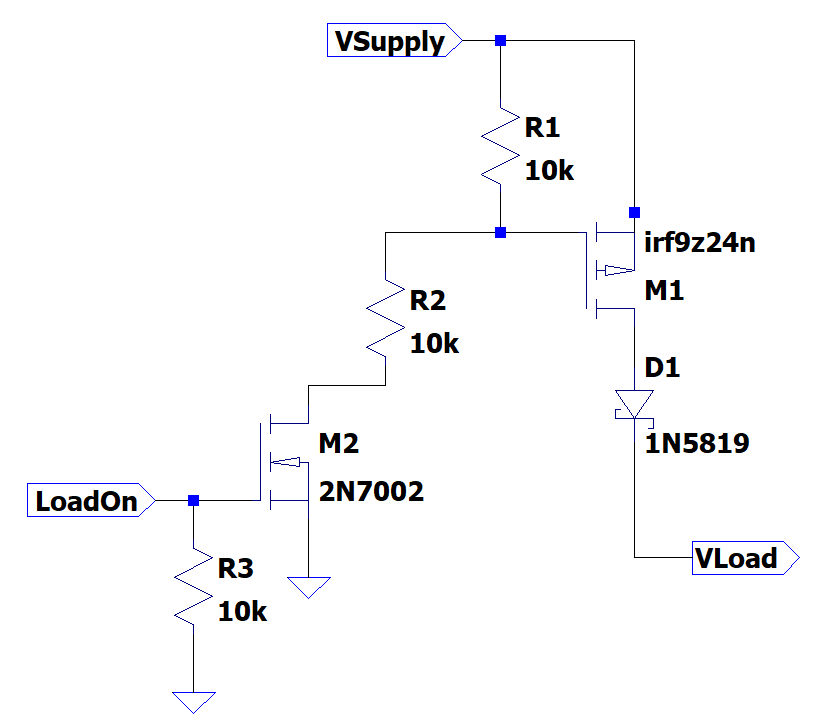
\includegraphics[scale=0.28]{Figures/Highside.png}
\caption{High side\textbf{} switch circuit}
\label{fig:high}
\end{figure}



%%%%%%%%%%%%%%%%%%%%%%%%%%%%%%%%%%%%%%%%%%%%%%%%%%%%%%%%%%%%%%%%%%%%%%%%%%%%%%%%%%%%%%%%%%%%%%%%%%%%%%%%%%%%%%%%%%%%%%%%%%%%%%%%%%%%%%%%%%%%%%%%%%%%%%%%%%%%%%%%%%%%%%%%%%%%%%%%%%%%%%%%%%%%%%%%%%%%%%%%%%
\newpage
\section{Over current protection}
From the battery's perspective, it will be able to discharge 60A for 5 seconds as an absolute maximum \cite{RS}. The battery also has a maximum recommended charging limit of 1.2A \cite{RS}. We will not be charging at 1.2A, we will be charging at approximately 400mA (I chose 300mA refer to \ref{sec:regulation}).

The load we are going to use will be made up of 5 ultra bright LEDs. The peak forward current of one of these LEDs is 100mA \cite{LED}. This means that for the peak case, just the load will use 500mA of current, however we will be designing for the typical 20mA per LED with current limiting resistors (refer to section \ref{sec:loswide}). This is then equated to 100mA for the entire load.

From the previously mentioned information we have 4 different current limit values. Two of these values are limits regarding the battery's limits and 2 are limits regarding what the circuit should charge/discharge. The fuse will be connected between the battery and the complete circuit, all current charging/discharging from the battery will flowing through the designed fuse.

The battery's limits are well above what the circuit will require, therefore the upper limit of the circuit charging will be used as the reference for the design. I then doubled the 400mA charging current to set the fuse for an abnormal condition. If 800mA of current flow then something is not working correctly and the battery should stop discharging. The closest fuse we have to this is 1A. 

%%%%%%%%%%%%%%%%%%%%%%%%%%%%%%%%%%%%%%%%%%%%%%%%%%%%%%%%%%%%%%%%%%%%%%%%%%%%%%%%%%%%%%%%%%%%%%%%%%%%%%%%%%%%%%%%%%%%%%%%%%%%%%%%%%%%%%%%%%%%%%%%%%%%%%%%%%%%%%%%%%%%%%%%%%%%%%%%%%%%%%%%%%%%%%%%%%%%%%%%%%
\newpage
\section{Undervoltage protection}
In the design below the concepts of a op amp voltage comparator is used. A comparator will amplify the difference of the two terminals.
\begin{figure}[!htb]
\centering
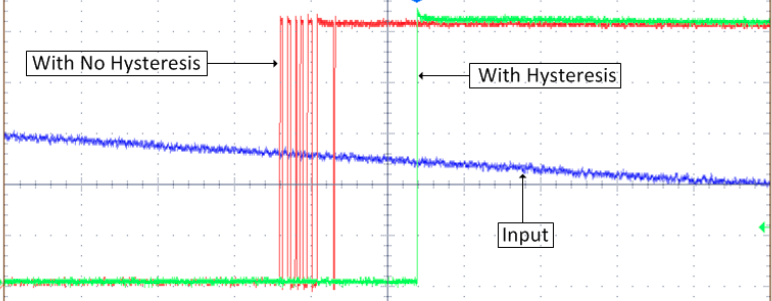
\includegraphics[scale=0.2]{./Figures/hyst}
\caption[{Op-Amp with hysteresis implemented compared with no hysteresis}]{Op-Amp with hysteresis implemented compared with no hysteresis \cite{TexHyst}}
\label{fig:hyst}
\end{figure}
A problem with the standard comparator op-amp configuration is that if a noisy signal is placed at the input of the op-amp it could cause the op amp output to switch between the two supply rails in a short period of time leading to a signal as can be seen in figure \ref{fig:hyst}. A op amp with hysteresis means that the op amp has positive feedback from the output and this causes the output of the op amp to switch from rail to rail at two voltages $V_{TU}$ and $V_{TL}$ , refer to \ref{fig:schmidt2}.




\subsection{5V rail}
In the circuit that was used in the final design an LM2940 regulator was chosen over a LM7805 regulator because of the respective drop out voltages of 0.5V \cite{TexReg} and 2V\cite{TexRegpos}. This is important because the voltage input to the regulator can be as low as 6V (battery terminal) and that would mean that the LM7805 would have a regulated voltage of below 5V. The LM7805 is able to output a maximum recommended amperage of 1.5A whereas the LM2904 only has a recommended output current of 1A \cite{TexReg}\cite{TexRegpos}. The LM2940 does have a typical quiescent current of 10mA which is ideal as we are designing for this current or less than 10mA \cite{TexReg}. 

\subsection{High-side switch}

%%%second part
The fundamental design is the same as in section \ref{sec:high}, the only difference is the lack of $R_2$ and the schottky diode. $R_2$ is not need to decrease the voltage $V_{GS}$ at the PMOS and no current flow restrictions are needed from the schottky diode. The high side switch is used at the position specified in figure \ref{fig:A3block}, it must be able to control the discharge of the battery but not restrict charging from the charging circuit. To ensure that this would not be an issue the reverse current of the PMOS was found in the respective data sheet to be -12A \cite{PMOS}.


\subsection{Voltage monitoring with hysteresis design}
 The positive supply rail of the op amps in this design will be connected to the 5V regulator and the negative supply rails will be grounded($V_{DD}$ and $V_{SS}$). When designing the input voltages to the op amp it was decided to step the voltages down using voltage division because if the battery terminal (max of 7.2V) is connected and a 0V is connected then the differential voltage maximum will be exceeded. The circuit that was built was based off the non inverting Schmidt trigger as can be seen in figure \ref{fig:schmidt2} \cite{Schmidt}.
 
 \begin{figure}[!htb]
 	\centering
 	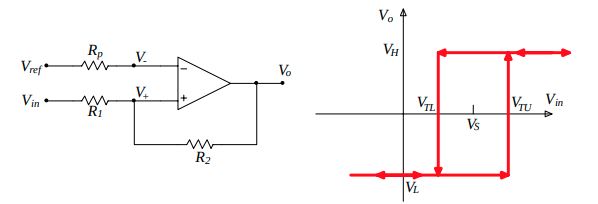
\includegraphics[scale=0.5]{./Figures/schmidt}
 	\caption[Non inverting Schmidt trigger]{Non inverting Schmidt trigger\cite{Schmidt}}
 	\label{fig:schmidt2}
 \end{figure}

  This configuration compares an input voltage with a constant reference voltage and the output will switch to the positive supply rail at an input voltage of $V_{TU}$ and to the negative supply rail at $V_{TL}$ (refer to \ref{fig:schmidt2}). A divided voltage from the 5V regulator is used as a reference voltage because it will remain "constant". The suitable $V_{ref-Schmidt}$ is calculated below and $V_{ref-Schmidt}$ is connected to a voltage follower op amp to prevent the positive feedback from affecting the input voltage. The battery voltage is divided to be 4.5V ($\frac{7.2*100}{100+60}$=4.5V) at the op amp terminal using $R_7$,$R_{10}$ and $R_8$(refer to figure \ref{fig:under}). With a battery terminal voltage of 6.2V the voltage at the op amp will be $V_{TU}=3.875$V and with 6V the voltage will be $V_{TL}=3.75$V. $V_L$ (approx zero volts) is the low output of the Schmidt trigger and $V_H$ is the high output of the Schmidt trigger(approx 5V). Equations below are for a non-inverting Schmidt trigger. \textbf{The equations are derived extensively in Appendix C}.



\begin{center}
	$\frac{V_{TU}-V_{TL}}{(V_{H}-V_L)}=\frac{R_1}{R_2}$  
\end{center}

\begin{center}
	
$	V_{REF}=\frac{V_{TL}\times (R_2)}{R_1+R_2}+\frac{V_{H}\times R_1}{R_1+R_2}$
\end{center}




Using the above equations the $\frac{R_1}{R_2}$ ratio is found to be $\frac{1}{40}$.$R_2$ is chosen to be 190k\textohm which results in $R_1$= 4.75k\textohm. The closest lab resistor is 4.7k\textohm. With our resistor values now defined $V_{REF}$ can be calculated to be 3.78V. The relevant voltage division can be found in figure \ref{fig:under}



\begin{figure}[!htb]
\centering
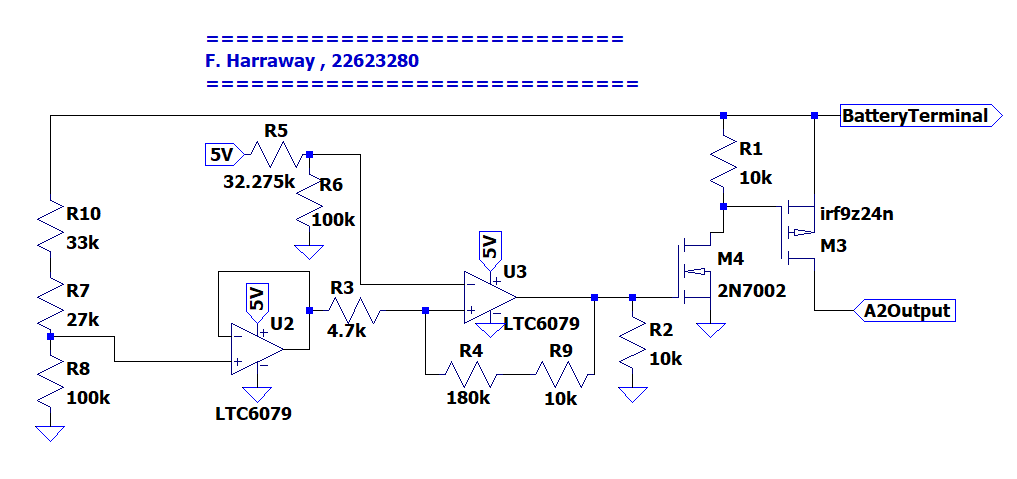
\includegraphics[scale=0.5]{./Figures/undervoltage}
\caption{Circuit diagram of under voltage circuit connected to the high side switch and the output of the previous assignment as well as the battery terminal}
\label{fig:under}
\end{figure}



\begin{table}[!htb]
	\centering
	\footnotesize
	\caption[Undervoltage circuit op amp requirements]{Undervoltage circuit op amp requirements \cite{MCP}}
	\begin{tabular}{lrrrr}
		\toprule
		& $Min$ &$Max$&$Designed$\\
		&[V]&[V]&[V]\\
		\midrule
		All op amps Difference between supply rails $V_{DD} - V_{SS}$ & -& 7  &5   \\
		U2 Common mode voltage $(\frac{V_+ + V_-}{2}-V_{SS})$ &  -0.3&5.3&3.75-4.5\\
		U2 Input voltages to $V_-$ and  $V_+$   &  -1    &6& 3.75-4.5 \\
		
		
		U3 Common mode voltage $(\frac{V_+ + V_-}{2}-V_{SS})$ &  -0.3&5.3&3.72-4.12\\
		U3 Input voltages to $V_-$ and $V_+$  &  -1    &6&0-4.51 \\
		U3 Differential Voltage $ (|V_+ - V_-|)$ & -& 7& 4.51   \\
		
		\bottomrule
	\end{tabular}
	\label{tab:MCPunder}
\end{table}

From table \ref{tab:MCPunder}, all op amps are operating within working ranges.


%%%%%%%%%%%%%%%%%%%%%%%%%%%%%%%%%%%%%%%%%%%%%%%%%%%%%%%%%%%%%%%%%%%%%%%%%%%%%%%%%%%%%%%%%%%%%%%%%%%%%%%%%%%%%%%%%%%%%%%%%%%%%%%%%%%%%%%%%%%%%%%%%%%%%%%%%%%%%%%%%%%%%%%%%%%%%%%%%%%%%%%%%%%%%%%%%%%%%%%%%%
\newpage
\section{Current sense}
The bidirectional current sense amplifier is an op amp that is setup internally as can be seen in figure \ref{fig:data}. This internal circuitry is necessary because the resistors used need to be very accurate in order for current sensing to be accurate \cite{utube}. Another reason that the tsc213 is being used over a conventional op amp is because this device has a absolute differential voltage of 26V and a common mode voltage range of $gnd-0.3V$ to 26V. This is important for us because we can have differential voltages of up to 7.2V ($7.2-0$) and common mode voltages of about 7.2V which would not work with the previously used MCP op amp. We do not want to step down the voltages as we did previously because it would not be accurate for the current measurements. The current sense amplifier will have its positive and negative inputs connected across a shunt resistor, the current sense amplifier will then amplify this difference by 50 (refer to \ref{fig:data}).



When designing the current sense amplifier the current range that will be used should be considered. The most current that should be discharged from the battery should be 100mA. The maximum that the battery should charge at is 400mA. The current range was then determined to be $-150mA<I_{range}<450mA$, the additional 50mA was added as a safety factor to ensure the tsc213 does not breach the 0-5V output range. We do not want to breach this range because it could damage the micro controller to which the output of the tsc213 will be connected. The output voltage range will be dependant on the differential voltage of the op amp and the reference voltage chosen (refer to eq \ref{eq:refeq}). The differential voltage will be dependant on the shunt resistance and the current through the shunt. The final circuit structure can be seen in figure \ref{subfig:c-s}.
\begin{equation}
    V_o=(R_{shunt}\times I_{shunt})\times50+V_{ref-cs}
    \label{eq:refeq}
\end{equation}
Using eq.\ref{eq:refeq} $R_{shunt}$ is designed to give an output voltage swing of 3V for the current sense amplifier.
\begin{center}
    $V_{swing}=((R_{shunt}\times 0.45)-(R_{shunt}\times -0.15))\times 50$. \ \ $R_{shunt}=0.1$\textohm 
\end{center}

This results in voltage range across the shunt of $-15mV<V_{shunt}<45mV$. With a 0V at $V_{ref-cs}$ the output range (using eq.\ref{eq:refeq}) would be -0.75V to 2.25V. This is not within 0V to 5V, this is where $V_{ref-cs}$ is used to place the output voltage into a desirable range. The minimum $V_{ref-cs}$ to get the output into the desired range would be 0.75V. The maximum $V_{ref-cs}$ that would place the maximum output voltage at 5V would be 2.75V (i.e. 5-2.25). The average of the maximum and minimum $V_{ref-cs}$ is then taken and found to be 1.75V. By doing this output voltage will be equally far from the upper and lower bounds of the 0V to 5V specification. To achieve this 1.75V the voltage from a 5V regulator is divided with resistors (refer to figure \ref{fig:A4circ}). \newline

To reduce the noise at the output a passive filter was designed and placed at the output of the TSC213. This can be seen in figure \ref{fig:A4circ}.The larger this capacitor the slower the response of the TSC213 output will be. If the value is too small then the output noise will not be sufficiently reduced. The passive filtering is needed because the 5V regulator as well as the 12V wall supply introduces a lot of noise into the system.

 \begin{figure}[!htb]
 \footnotesize
 \centering
    \begin{subfigure}[]{0.42\textwidth}
              \centering
  		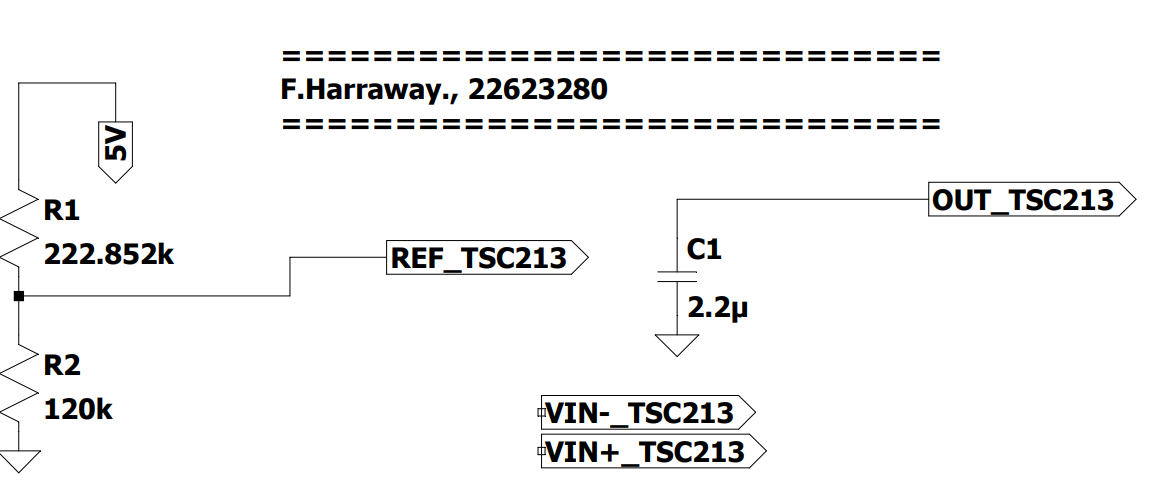
\includegraphics[width=1\linewidth]{./Figures/A4circ}
		    \caption{} \label{fig:A4circ}
     \end{subfigure}
     \begin{subfigure}[]{0.5\textwidth}
             \centering
  		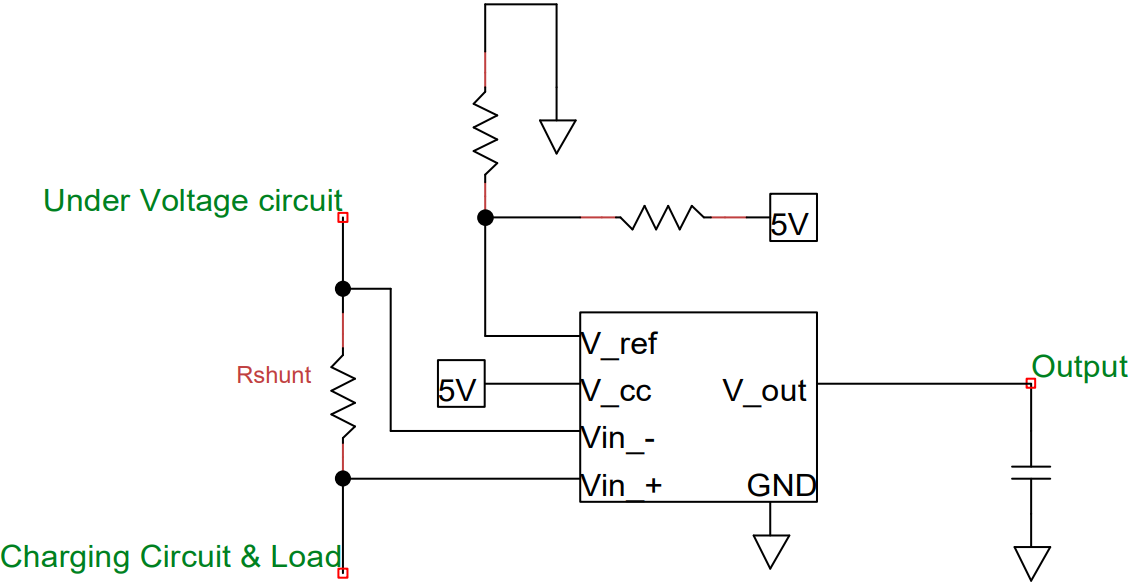
\includegraphics[width=1\linewidth]{./Figures/currentSense}
		   \caption{ } \label{subfig:c-s}
     \end{subfigure}
   \caption[{Fuse Characteristics}]{Current sense circuitry   (a) LT Spice current sense circuit (b)  Current sense circuit }
    \label{fig:C-S}
 \end{figure}




%%%%%%%%%%%%%%%%%%%%%%%%%%%%%%%%%%%%%%%%%%%%%%%%%%%%%%%%%%%%%%%%%%%%%%%%%%%%%%%%%%%%%%%%%%%%%%%%%%%%%%%%%%%%%%%%%%%%%%%%%%%%%%%%%%%%%%%%%%%%%%%%%%%%%%%%%%%%%%%%%%%%%%%%%%%%%%%%%%%%%%%%%%%%%%%%%%%%%%%%%%
\newpage
\section{Low Side Switch and Load}
\label{sec:loswide}
\label{sec:loadcontrol_lit}
In this design notable factors that will affect the design will be outlined. The load that will be used is made up of 5 LEDs that will be designed in such a way so that together 100mA is drawn. The NMOS we are going to use is able to sink a maximum continuous drain current of 200mA \cite{NData}. A low side switch means that the "switching element" is place in between ground and the load. This can be seen in figure \ref{fig:loadcirc}.

\label{sec:loadcontrol_design}
Because 100mA is the maximum current a 2n7000 NMOS chip was deemed enough to be used as a switch for the load. To "turn on" the NMOS a 5V control signal will be used. To ensure that the gate of the NMOS can not float a pull down resistor will be used. For a drain current of 100mA, according to the data sheet the $V_{DSon}$ voltage will be approximately 0.2V for a $V_{gs}$ of 5V \cite{NData}. The LED we are using has a typical forward bias voltage of 3.2V at 20mA \cite{LED}. To limit the current to 20mA ($7.2V-20mA*R_{limit}=3.2V+0.2V$) a resistor of 190\textohm \ would be ideal ,but only 220\textohm's are available in the labs. The LEDs will be in series with the current limiting resistor. The LED-resistor units will then be placed in parallel to each other (refer to figure \ref{fig:loadcirc}).

\begin{figure}[!htb]
    \centering
    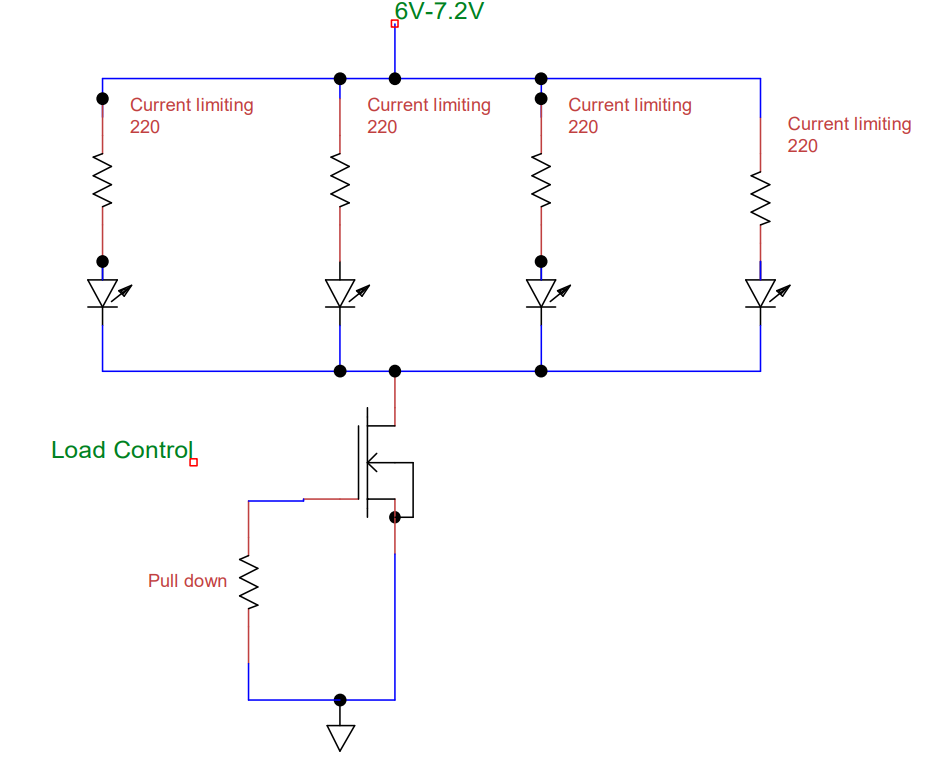
\includegraphics[width=0.4\linewidth]{Figures/loadCircuit.png}
    \caption{Load circuitry with low side switch implemented}
    \label{fig:loadcirc}
\end{figure}

\newpage
\section{Supply voltage measurement}
The Supply voltage of supply will vary from voltages of zero volt to just below 23V. To measure the supply measurement needs to converted to a voltage between zero and five volts in order for the arduino beetle to successfully read a voltage without breaking. There should be a boundary between 5V and the maximum converted voltage. To implement this a maximum voltage of 24V is designed for instead of 23V. One of the two possible supplies, the AC wall plug will introduce noise into the circuit (50Hz from the mains). This noise will likely be 50Hz which will be designed for adequately using a low pass RC filter.


\begin{center}
	$\frac{R_{10}}{R_{10}+R_9}\times24V=5V$
\end{center}
If $R_9$ is chosen to be 100k\textohm \ $R_{10}$ will be 26.3k\textohm.

\begin{equation}
f_c=\frac{1}{2\times pi\times R\times C}
\label{eq:freq}
\end{equation}
To prevent the noise of the ac wall plug from interfering with the measurement the low pass cut off filter is designed to cut off at half of 50Hz to ensure a cleaner signal. The capacitor is chosen to be 200nF. Cutting off at a lower frequency would get rid of more noise  and attenuate 50Hz noise better, however the rise time is dependant on the cut off frequency. $T_r \approx \frac{0.35}{f_c}$. For this reason the cut off frequency is not designed too low.  As an example the error that a 100mV offset on the input to the ADC will have is calculated as $\frac{100mV\times 26}{126}= V_{error}$, $V_{error}$ is then equal to 0.48V. This indicates the need for a filter.

Using eq.\ref{eq:freq} with a chosen capacitor of 200nF the required resistance for a 25Hz cut off is found to be 32k\textohm.

\begin{figure}[!htb]
	\centering
	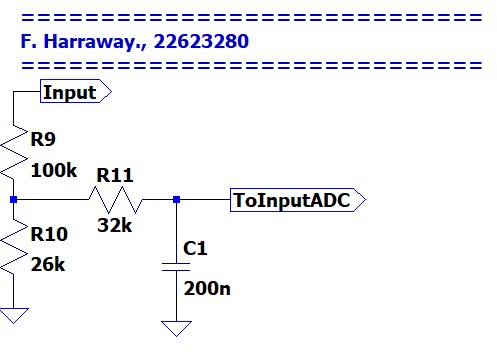
\includegraphics[width=0.26\linewidth]{Figures/A6/Supsig.jpg}
	\caption{Supply measurement circuit}
	\label{fig:supcirc}
\end{figure}


\newpage

\section{Battery voltage measurement}
In this design the battery voltage will be go through a signal conditioning process to make it readable from the perspective of an ADC. The ADC we are going to use requires a voltage between 0 and 5V. The battery voltage will vary between 6V and 7.2V if the complete system is working as designed. 

For the purpose of the design an additional 0.3V will be extended on to either side of the boundaries to give a margin for error (5.7V to 7.5V).  Using Op Amps the battery voltage will be designed to vary linearly with an output swing of 4.3V (0.5V to 4.8V). As the battery voltage increases the ADC voltage will increase. The ADC output is less than five volts in order to prevent damage to the ADC as well as the op amps. The chosen resistors are chosen to be bigger than 20k\textohm \ in order to minimise current drawn from the battery and the five volt regulator. To fit op amp spec requirements the input voltage is divided with resistors to be  four volts at the maximum designed voltage of 7.5V  as can be see in figure \ref{fig:batcirc}, this will result in a voltage of 3.04V when the battery voltage is 5.7V.

\begin{figure}[!htb]
	\centering
	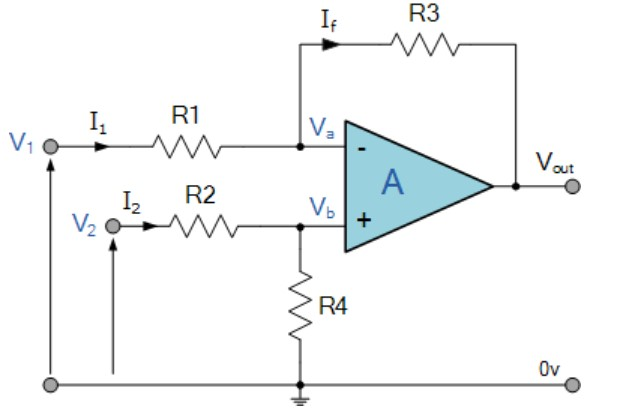
\includegraphics[width=0.27\linewidth]{Figures/A6/difamp.jpg}
	\caption[Differential amplifier op amp setup]{Differential amplifier op amp setup\cite{difAmp} }
	\label{fig:difamp}
\end{figure}

To achieve the differential amplifier setup from figure \ref{fig:difamp} is used. In this design $R_1$=$R_2$ and $R_3$=$R_4$ \cite{difAmp}. The corresponding equation is as seen in equation \ref{eq:diff}.  $V_1$ will be used as the reference voltage and $V_2$ will be our input from the battery. \textbf{The derivation can be found in Appendix D \ref{fig:derive}}.

\begin{equation}
	V_{out}=\frac{R_3}{R_1}\times(V_{2(bat)}-V_{1(ref)}) 
	\label{eq:diff}
\end{equation}

Using eq.\ref{eq:diff}, $V_{1(ref)}$ and the gain is solved for simultaneously by setting the equations for the scenarios when the battery voltage is 7.5V and 5.7V.

\begin{center}
	 $4.8V=\frac{R_3}{R_1}\times(4V-V_{1(ref)}) \ \ \ \ \ \ \ \ 0.5=\frac{R_3}{R_1}\times(3.04V-V_{1(ref)}) $\newline 
	
	$\frac{4.8V}{(V_{1(ref)}-4V)}=\frac{0.5V}{(V_{1(ref)}-3.04V)}  \ \ \ \ \ \ \ \ V_{1(ref)}=2.93V \ \ \ \ \ \ \frac{R_3}{R_1}=4.48$\newline
\end{center}


$R_3$ is then chosen to be 100k\textohm. $R_1$ is the calculated to be 22.32k\textohm. Both $V_1$ and $V_2$ need to be divided to a lower voltages 2.93V and four volts (when battery is at 7.5V), the relevant resistors for the voltage division can be seen in figure \ref{fig:batcirc}.  $V_1$ requires a buffer in between the divided battery voltage and the differential op amp to prevent the negative feedback from interfering with the input voltage. $V_2$ also requires a buffer because otherwise $R_2$ and $R_4$ will the change the effective voltage division and 2.93V would not be achieved. 

\begin{figure}[!htb]
	\centering
	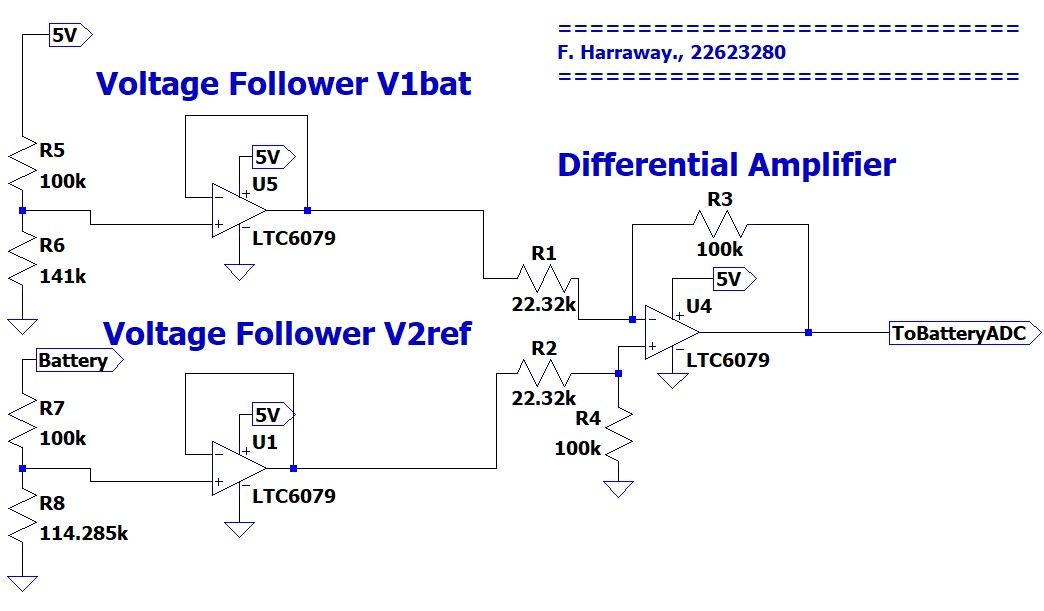
\includegraphics[width=0.5\linewidth]{Figures/A6/Batterysig.jpg}
	\caption{Battery measurement circuit}
	\label{fig:batcirc}
\end{figure}


\begin{table}[!htb]
	\centering
	\footnotesize
	\caption[Battery voltage measurement circuit op amp requirements]{Battery voltage measurement circuit op amp requirements \cite{MCP}}
	\begin{tabular}{lrrrr}
		\toprule
		& $Min$ &$Max$&$Designed$ $range / value$\\
		&[V]&[V]&[V]\\
		\midrule
		All op amps Difference between supply rails $V_{DD} - V_{SS}$ & -& 7  &5   \\
		
		U1 Common mode voltage $(\frac{V_+ + V_-}{2}-V_{SS})$ &  -0.3&5.3&3-4\\
		U1 Input voltages to $V_-$ and $V_+$  &  -1    &6& 3-4 \\
		
		U5 Common mode voltage $(\frac{V_+ + V_-}{2}-V_{SS})$ &  -0.3&5.3&2.92\\
		U5 Input voltages to $V_-$ and $V_+$ &  -1    &6& 3-4 \\
		
		
		U4 Common mode voltage $(\frac{V_+ + V_-}{2}-V_{SS})$ &  -0.3&5.3&2.48-3.28\\
		U4 Input voltages to $V_-$ and $V_+$  &  -1    &6&2.48-3.28 \\
		U4 Differential Voltage $ (|V_+ - V_-|)$ & -& 5&  3.28  \\
		
		\bottomrule
	\end{tabular}
	\label{tab:MCPbat}
\end{table}

From table \ref{tab:MCPbat}, all op amps are operating within working ranges.
%%%%%%%%%%%%%%%%%%%%%%%%%%%%%%%%%%%%%%%%%%%%%%%%%%%%%%%%%%%%%%%%%%%%%%%%%%%%%%%%%%%%%%%%%%%%%%%%%%%%%%%%%%

\section{Ambient light sensor circuitry}
The LDR will be used to produce a voltage that will fall within the boundary of zero to five volts in order to work correctly with an ADC when "measuring" the light. In direct sunlight the LDR had a resistance of as little as 500\textohm and in complete darkness a resistance of greater than 1M\textohm \ was measured.  To get a voltage between zero and five volts, the voltage from the 5V regulator is divided as can be seen in figure \ref{fig:LDR}. This means that unless the regulator exceeds its values the zero to five volt range of the LDR circuit will not be breached. In the labs the highest "light" measured LDR resistance is 15k\textohm. When we are at this point the ADC output is designed to have a voltage of 2.5V. This 2.5V will be used in the next section.


\begin{figure}[!htb]
	\centering
	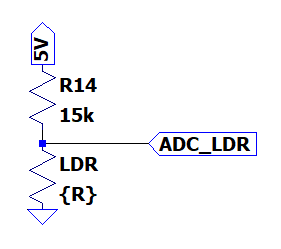
\includegraphics[width=0.25\linewidth]{Figures/A7/LDRcirc.png}
	\caption{Light measuring circuit}
	\label{fig:LDR}
\end{figure}

\section{LED load control design }

The following design will consist of 


\begin{table}[!htb]
	\centering
	\footnotesize
	\caption[Truth table of load control]{Truth table of load control}
	\begin{tabular}{lrrrr}
		\toprule
		$PWM$&$Load Control$&$Light Condition$&$Load LED$&$Pilot LED$\\
		&[0-off/1-on]&[0-Light/1-Dark]&[0-off/1-on]&[0-off/1-on]&[0-off/1-on]\\
		\midrule
		1&0&0&0&0\\
		1&0&1&0&1\\
		1&1&0&0&0\\
		1&1&1&1&0\\
		\bottomrule
	\end{tabular}
	\label{tab:truthtab}
\end{table}

\subsection{Pilot light control design}





